\iffalse
\documentclass[journal,12pt,twocolumn]{IEEEtran}
\usepackage{setspace}
\usepackage{gensymb}
\usepackage{xcolor}
\usepackage{caption}
\singlespacing
\usepackage{siunitx}
\usepackage[cmex10]{amsmath}
\usepackage{mathtools}
\usepackage{hyperref}
\usepackage{amsthm}
\usepackage{mathrsfs}
\usepackage{txfonts}
\usepackage{stfloats}
\usepackage{cite}
\usepackage{cases}
\usepackage{subfig}
\usepackage{longtable}
\usepackage{multirow}
\usepackage{enumitem}
\usepackage{mathtools}
\usepackage{listings}
\usepackage{tikz}
\usetikzlibrary{shapes,arrows,positioning}
\usepackage{circuitikz}
\let\vec\mathbf
\DeclareMathOperator*{\Res}{Res}
\renewcommand\thesection{\arabic{section}}
\renewcommand\thesubsection{\thesection.\arabic{subsection}}
\renewcommand\thesubsubsection{\thesubsection.\arabic{subsubsection}}

\renewcommand\thesectiondis{\arabic{section}}
\renewcommand\thesubsectiondis{\thesectiondis.\arabic{subsection}}
\renewcommand\thesubsubsectiondis{\thesubsectiondis.\arabic{subsubsection}}
\hyphenation{op-tical net-works semi-conduc-tor}

\lstset{
language=Python,
frame=single, 
breaklines=true,
columns=fullflexible
}
\begin{document}
\theoremstyle{definition}
\newtheorem{theorem}{Theorem}[section]
\newtheorem{problem}{Problem}
\newtheorem{proposition}{Proposition}[section]
\newtheorem{lemma}{Lemma}[section]
\newtheorem{corollary}[theorem]{Corollary}
\newtheorem{example}{Example}[section]
\newtheorem{definition}{Definition}[section]
\newcommand{\BEQA}{\begin{eqnarray}}
\newcommand{\EEQA}{\end{eqnarray}}
\newcommand{\define}{\stackrel{\triangle}{=}}
\newenvironment{amatrix}[1]{%
  \left(\begin{array}{@{}*{#1}{c}|c@{}}
}{%
  \end{array}\right)
}
\newcommand{\myvec}[1]{\ensuremath{\begin{pmatrix}#1\end{pmatrix}}}
\newcommand{\myaugvec}[2]{\ensuremath{\begin{amatrix}{#1}#2\end{amatrix}}}
\newcommand{\mydet}[1]{\ensuremath{\begin{vmatrix}#1\end{vmatrix}}}
\bibliographystyle{IEEEtran}
\providecommand{\nCr}[2]{\,^{#1}C_{#2}} % nCr
\providecommand{\nPr}[2]{\,^{#1}P_{#2}} % nPr
\providecommand{\mbf}{\mathbf}
\providecommand{\pr}[1]{\ensuremath{\Pr\left(#1\right)}}
\providecommand{\qfunc}[1]{\ensuremath{Q\left(#1\right)}}
\providecommand{\sbrak}[1]{\ensuremath{{}\left[#1\right]}}
\providecommand{\lsbrak}[1]{\ensuremath{{}\left[#1\right.}}
\providecommand{\rsbrak}[1]{\ensuremath{{}\left.#1\right]}}
\providecommand{\brak}[1]{\ensuremath{\left(#1\right)}}
\providecommand{\lbrak}[1]{\ensuremath{\left(#1\right.}}
\providecommand{\rbrak}[1]{\ensuremath{\left.#1\right)}}
\providecommand{\cbrak}[1]{\ensuremath{\left\{#1\right\}}}
\providecommand{\lcbrak}[1]{\ensuremath{\left\{#1\right.}}
\providecommand{\rcbrak}[1]{\ensuremath{\left.#1\right\}}}
\theoremstyle{remark}
\newtheorem{rem}{Remark}
\newcommand{\sgn}{\mathop{\mathrm{sgn}}}
\newcommand{\rect}{\mathop{\mathrm{rect}}}
\newcommand{\sinc}{\mathop{\mathrm{sinc}}}
\providecommand{\abs}[1]{\left\vert#1\right\vert}
\providecommand{\res}[1]{\Res\displaylimits_{#1}} 
\providecommand{\norm}[1]{\left\Vert#1\right\Vert}
\providecommand{\mtx}[1]{\mathbf{#1}}
\providecommand{\mean}[1]{E\left[ #1 \right]}
\providecommand{\fourier}{\overset{\mathcal{F}}{ \rightleftharpoons}}
\providecommand{\ztrans}{\overset{\mathcal{Z}}{ \rightleftharpoons}}
\providecommand{\system}[1]{\overset{\mathcal{#1}}{ \longleftrightarrow}}
\newcommand{\solution}{\noindent \textbf{Solution: }}
\providecommand{\dec}[2]{\ensuremath{\overset{#1}{\underset{#2}{\gtrless}}}}
\let\StandardTheFigure\thefigure
\def\putbox#1#2#3{\makebox[0in][l]{\makebox[#1][l]{}\raisebox{\baselineskip}[0in][0in]{\raisebox{#2}[0in][0in]{#3}}}}
     \def\rightbox#1{\makebox[0in][r]{#1}}
     \def\centbox#1{\makebox[0in]{#1}}
     \def\topbox#1{\raisebox{-\baselineskip}[0in][0in]{#1}}
     \def\midbox#1{\raisebox{-0.5\baselineskip}[0in][0in]{#1}}

\vspace{3cm}
\title{Line Assignment}
\author{Gautam Singh}
\maketitle
\bigskip

\begin{abstract}
    This document contains the solution to Question 24 of Exercise 4 
    in Chapter 10 of the class 11 NCERT textbook.
\end{abstract}

\begin{enumerate}
\fi
		We first find the coordinates of the intersection of \eqref{eq:chapters/11/10/4/24/L1}
    and \eqref{eq:chapters/11/10/4/24/L2}. Using the augmented matrix and row reduction methods,
    \begin{align}
        \myaugvec{2}{2&-3&-4\\3&4&5} &\xleftrightarrow[]{R_2\rightarrow2R_2-3R_1} 
        \myaugvec{2}{2&-3&-4\\0&17&22} \\
                      &\xleftrightarrow[]{R_1\rightarrow17R_1+3R_2} \myaugvec{2}{17&0&-1\\0&17&22} \\
                      &\xleftrightarrow[]{\substack{R_1\rightarrow\frac{R_1}{17}\\R_2\rightarrow\frac{R_2}{17}}} \myaugvec{2}{1&0&-\frac{1}{17}\\0&1&\frac{22}{17}}
        \label{eq:chapters/11/10/4/24/intersect}
    \end{align}
    the intersection of the lines is
    \begin{align}
        \vec{A} = \frac{1}{17}\myvec{-1\\22}
    \end{align}
    Clearly, the man should follow the path perpendicular to \eqref{eq:chapters/11/10/4/24/L3} from
    $\vec{A}$ to reach it in the shortest time. The normal vector 
    of \eqref{eq:chapters/11/10/4/24/L3} is 
    \begin{align}
        \vec{m} = \myvec{6\\-7}
        \label{eq:chapters/11/10/4/24/L3-norm}
    \end{align}
    which is consequently the direction vector of the required line. Therefore, 
    the required normal vector is given by
    \begin{align}
        \vec{n} = \myvec{7\\6}
        \label{eq:chapters/11/10/4/24/L4-norm}
    \end{align}
    and hence, the equation of the line is
    \begin{align}
        \vec{n}^\top\vec{x} &= \vec{n}^\top\vec{A} \\
        \implies \myvec{7&6}\vec{x} &= \frac{1}{17}\myvec{7&6}\myvec{-1\\22} = \frac{125}{17}
        \label{eq:chapters/11/10/4/24/L4}
    \end{align}
		See Fig. \ref{fig:chapters/11/10/4/24/crossing}. In this figure $\vec{F}$ represents 
    the foot of the prependicular drawn from $\vec{A}$ onto \eqref{eq:chapters/11/10/4/24/L3}.
    \begin{figure}[!ht]
        \centering
        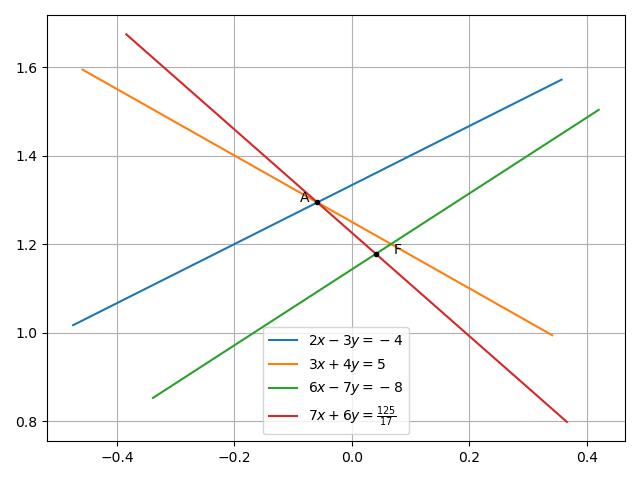
\includegraphics[width=\columnwidth]{chapters/11/10/4/24/figs/crossing.png}
        \caption{AF is the required line.}
        \label{fig:chapters/11/10/4/24/crossing}
    \end{figure}
